%!TEX root = ../main.tex
\section{Registration Algorithm}

This section describes the presented algorithm.
We first pre-register all individual scans to align them in one global coordinate system.
Then, planes are extracted from this global scan model.
The key to improving map quality is to find a model for each individual scan, where each point is correctly identified to belong to one of the globally extracted planes.
Then, each scan is optimized by finding a 6D pose-transformation that minimizes the distance of each correspondence.
Note that all of this takes place on a reduced version of the scan, i.e. an octree based reduction where each voxel is only allowed to have a certain amount of points.
This ensures a homogenous point density, which is favourable for the error function.
It also decreases runtime, while preserving the planar features of the environment. 
 
Consider a line scan as the smallest chunk of range data we obtain from the scanner device driver.
In the case of a SICK LMS1xx it is a line, and in case of a Livox scanner it has a flower shape.
More details are provided in the following sections.
We start with transforming each line scan into the project coordinate system, which is defined by the pose of the first acquired line scan.
%
For map improvement, the individual scans need to be registered to another. 
We propose an algorithm that consists of multiple steps outlined in algorithm~\ref{algo:registration-algorithm}. 
Based on ideas described in~\cite{Borrmann2010} we first pre-register the scans and then further improve the overall map by exploiting the fact that human-made environments often consist of planes. 
We then find the planes in the pre-registered point cloud and then optimize the poses associated with the scans to minimize the distance of all points to their respective planes. 

\begin{algorithm}
    \SetAlgoLined
    \KwResult{A corrected map and 6D path.}
    1. Pre-register the scans\;
    2. Extract planes from the registered map globally\;
    3. Further improve map by solving the optimization that minimizes the distance of all points to their respective planes\;
    \caption{Registration algorithm for man-made environments}
    \label{algo:registration-algorithm}
\end{algorithm}

\subsection{Pre-Registration}

For the plane extraction the linescans need to be transformed into the project coordinate system.
Various pre-registration methods are suitable for this.
The most simple method is to use the data from an intertial measurement unit for a coarse alignment.
Alternative solutions combine multiple linescans into a metascan and perform registration methods known from terrestrial laser scanning \todo{add source here} or use a small number of iterations of continuous-time SLAM approaches such as the one presented in~\cite{REMSEN2013}.
This yields maps that can be used for plane registration and hence a point-to-plane correspondences based registration.

\subsection{Plane Extraction}

After having done the pre-registration, the scans are aligned well enough to make statements about the potential planes in the environment.
We extract planes only once from the global scan model, or a portion of that global scan model.
The first few line scans, e.g. the first half of the global model, is sufficient for plane extration.
This is because within the initial movements of the robot system, pose error has not accumulated for very long, resulting in a less dense, yet less distorted representation of the environment.
For mobile robots this yields a quite consistent strategy for global plane extraction, since all the subsequent scans (where pose error keeps accumulating) get matched with the initial planar representation.
However, especially for large datasets, it is necessary to update the global plane model multiple times while establishing point to plane correspondences.  
Currently, this is not done, and is one of the primary objectives for future works.

To find the planes in the environment, a Randomized Hough transform (RHT) with an accumulator ball as described in~\cite{3DRESEARCH2011} is used as this method prefers dominant planes such as the building structure over smaller planar surfaces.
The RHT is combined with a region growing approach, similar plane merging, and a flatness filter that is based on principal component analysis (PCA).
Once a plane is identified, we calculate the convex hull of that plane, representing the extent in all directions. 
This way, large planar structures such as walls or the ceiling get identified.
Note that smaller, non-perpendicular planes such as doors or cupboards potentially get identified, too, if they pass the PCA filter.

In the next subsection, the Hesse-normal form of the plane is required.
For an ideal plane the orthogonal distance from the origin $\rho_{\mathcal{P}_k}$ is computed via $\vec{n}_{\mathcal{P}_k}\cdot\vec{p}_i$, where $\vec{p}_i = \begin{bmatrix}x_i&y_i&z_i\end{bmatrix}^T$ is an arbitrary point on the plane and $\vec{n}_{\mathcal{P}_k} = \begin{bmatrix}n_{\mathcal{P}_k}^x&n_{\mathcal{P}_k}^y&n_{\mathcal{P}_k}^z\end{bmatrix}^T$ is the normal vector of that plane.
To find this point, we use the convex hull, as it is defined by the points that lie on the plane with the furthest distance to one another.
We choose the center point of the convex hull of the plane as $\vec{a}_{\rho_k}$.

\subsection{Point-to-Plane Correspondences}\label{sec:point-to-plane-correspondences}


There are many ways of solving the segmentation problem of assigning each point to a plane. They are often based on the RANSAC method \cite{Honti2018}, \cite{Gaspers2011} but also deep learning approaches \cite{Engelmann2018} have been successful.
The quality of the preregistration directly influences the quality of the plane detection and therefore the quality of the final registration result.
We assume small enough errors in pre-registration to allow for plane detection.
We employ two distance models to represent the distance from a point to a plane, and combine them with a local planar clustering (LPC) approach to establish point-to-plane correspondences.

\subsubsection{Distance Models}

\begin{figure*}
	\centering
	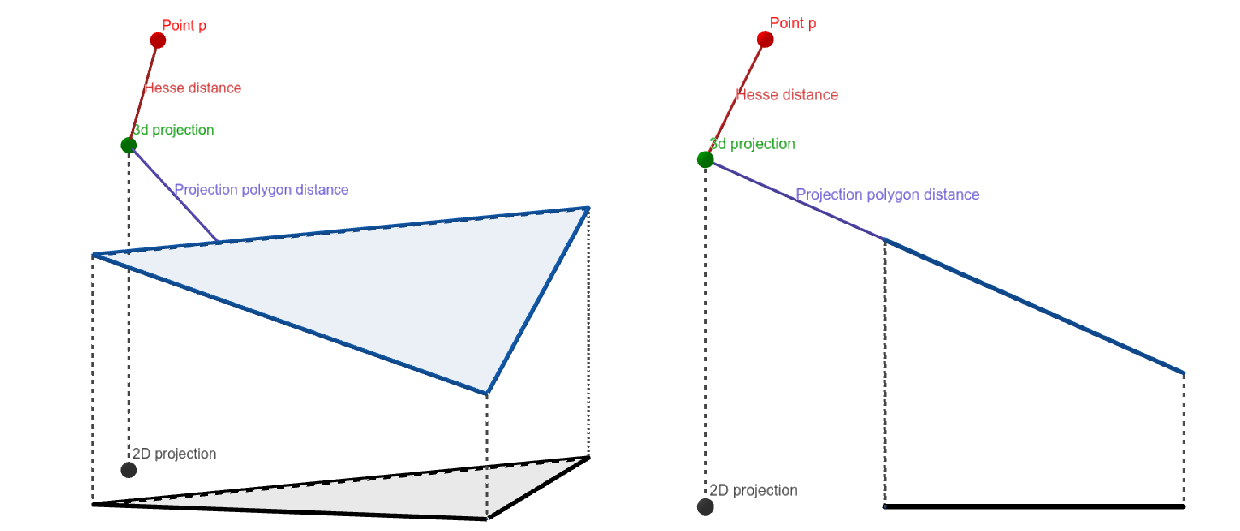
\includegraphics[width=\textwidth]{images/project}
	\caption{Illustration of the Hesse- and polygon projection distance. The point p (red) gets projected onto the infinitely extending global plane. Both the point projection (green) and the global planes convex hull (blue) get projected into 2D space (grey). The Hesse distance, i.e. the shortest distance to the infinitely extending plane (red), is shown as well as the minimum distance from the 2D point projection to the polygon (purple).}
	\label{fig:proj}
\end{figure*}

The Hesse-normal form describes the distance from the $i$-th transformed point $T(\vec{p}_i)$ to infinitely extending, $k$-th plane in 3D vector space
\begin{equation}\label{eq:hesse}
	D_{h}^{i,k} = \vec{n}_{\mathcal{P}_k} \cdot \left[ T(\vec{p}_i) - \vec{a}_{\mathcal{P}_k} \right] ,
\end{equation}
with normal $\vec{n}_{\mathcal{P}_k}$ and supporting point $\vec{a}_{\mathcal{P}_k}$ of the $k$-th plane.
The distance $D_{h}^{i,k}$ of the $i$-th point to the $k$-th plane reflects the length of the line segment, constructed from the $i$-th point to its projection on the $k$-th plane.
Therefore, by definition the line segment is parallel to the normal vector of the plane.
Thus, the $i$-th points projection $\widetilde{T}(\vec{p}_i)$ onto the $k$-th plane, which is required later, is easily calculated by shifting the point against normal direction:
\begin{equation}\label{eq:projection}
	\widetilde{T}(\vec{p}_i) = T(\vec{p}_i) - D_{h}^{i,k} \vec{n}_{\mathcal{P}_k}
\end{equation}

The simplicity of the Hesse distance is at contrast with its inability to take the extent of the plane into account.
Therefore, a second distance model is introduced: the polygon projection distance (PPD).
The convex hull represents the extend of a plane by forming a polygon with the outer most points that are assigned to a given plane. 
It is able to represent the expansion of the plane in all directions, and thus is utilized as a distance model.
To find the PPD, first a corresponding point gets projected onto the infinitely extending plane representation given by the Hesse form, i.e. $\widetilde{T}(\vec{p}_k)$ is found from eq.~\eqref{eq:projection} (green point in~\ref{fig:proj}).
Then, the 3D polygon, i.e. the points that make up the convex hull, as well as the corresponding 3D point projection, are projected again into a 2D vector space, using the maximal component of the normal vector of the plane.
E.g. in figure~\ref{fig:proj}, the blue planes normal vector has its mayor component in z-direction (upwards), thus the projection polygon distance is calculated in the xy-plane.
Using the maximum of the absolute magnitude of the normal vector ensures that the most sensible 2D projection is used for every direction.
Sunday et al.~\cite{pga} presents an optimal algorithm to check whether the point projection lies inside the polygon in 2D. 
If the point is inside the polygon, its PPD is set to zero.
If, however, the point is outside the polygon, the shortest distance to the polygon is calculated by looking at the minimum distance of the $i$-th point to each line segment, making up the convex hull of the $k$-th plane in 3D.
Let the polygon $P_k$ be made up of line segments $s_{m, j}$.
The line segment $s_{m, j}$ consists of the points $p_m$ and $p_j$.
The line segment is parameterized by
\begin{equation}
\label{eq:line}
	s_{m, j}(t) = p_m + t \cdot \left( p_j - p_m \right) ,  
\end{equation}
where $t \in \left[ 0, 1 \right]$. 
We set up a distance function, which measures the distance from the query point $p_i$ to an arbitrary point on the line segment.
\begin{equation}
	\label{eq:dist}
	d_{m, j}(t) = \lVert s_{m, j}(t) - p_i \rVert 
\end{equation} 
It is now possible to find the shortest distance to the line segment by finding the argument of the function that minimizes this distance.
Therefore, we set
\begin{equation}
	\pardiff{t} d_{m, j}(t)^2 \overset{!}{=} 0 ,
\end{equation}  
resulting in 
\begin{equation}
	t_0 = \frac{\left( p_j - p_m \right) \cdot \left( p_i - p_m \right)}{\left( p_j - p_m \right)^2} .
\end{equation}
Note the possibility of $t_0 \notin \left[ 0, 1 \right]$. 
In that case, the projection of the point $p_i$ onto the line given by eq.~\ref{eq:line} is not between $p_j$ and $p_m$. 
Instead, its projection onto the line falls outside of the segment.
By constraining $t_0$ we get 
\begin{equation}
\label{eq:minmax}
	\hat t = \min \left( \max \left( t_0, 0\right) , 1 \right) ,
\end{equation}
which is the argument that gives the shortest distance to the line segment, when inserted to eq. \ref{eq:dist}.
We find the PPD from the point $p_i$ to the polygon $P_k$ by calculating the minimum shortest distance over all line segments that make up the polygon.  

\subsubsection{Local Planar Clustering}

The presented algorithm employs LPC on each individual line scan.
The idea is to find planar features utilizing an optimized approximate k nearest neighbor (AKNN) search for normal calculation as in~\cite{aknnbbs}.
Thus, normals are calculated for every point in the respective line scan.
Then, the local normal model is combined with a region growing approach.
The region growing is implemented by storing the k-nearest neighbors in a queue, which represents the iteration order of the clustering algorithm.
A region grows if one of these neighbors has a distance shorter then a threshold $d_{growth}$ and additionally has a similar normal.
We define similarity of two normals via the angle between them, which is:
\begin{equation}
\label{eq:smallestalpha}
	\alpha(\vec{n}_1, \vec{n}_2) = \arccos(\vec{n}_1 \cdot \vec{n}_2) \; .
\end{equation}
However, the \textit{smallest} angle between two \textit{normal} vectors is 
\begin{equation}
\label{eq:alphahat}
\hat \alpha(\vec{n}_1, \vec{n}_2) = 
\begin{cases}
	2\pi - \alpha(\vec{n}_1, \vec{n}_2) & \text{if  } \alpha(\vec{n}_1, \vec{n}_2) > \frac{3}{2} \pi \\
	\alpha(\vec{n}_1, \vec{n}_2) - \pi & \text{if  } \alpha(\vec{n}_1, \vec{n}_2) > \pi \\
	\pi - \alpha(\vec{n}_1, \vec{n}_2) & \text{if  } \alpha(\vec{n}_1, \vec{n}_2) > \frac{\pi}{2} 
\end{cases}
\; ,
\end{equation}
because the opposing normals $-\vec{n}_1$ and $-\vec{n}_2$ always have to be considered, since they correspond to the same plane.
We say that two normals are similar if the angle $\hat \alpha$ from eq. \ref{eq:alphahat} is smaller than a threshold $\epsilon_{\alpha}$. 

Planar areas like walls are therefore connected in one large cluster, while non-feature parts, i.e. non-planar or detached parts of the scan will have their own, smaller cluster.
Finally the clusters are filtered in two steps.
First, to combine clusters that are similar, i.e. have a short distance ($d_{growth}$) to each other and similar mean normals (similarity defined as before).
Second, to filter out all clusters that contain non-feature points.
Since all the non-feature points belong to small clusters, the presented algorihtm does this by putting a minimum threshold $N_{c,min}$ on the cluster size.
Figure \ref{fig:clustering} shows this concept on the real world dataset described later in section \ref{sec:experimentalSetup}.

\begin{figure*}
	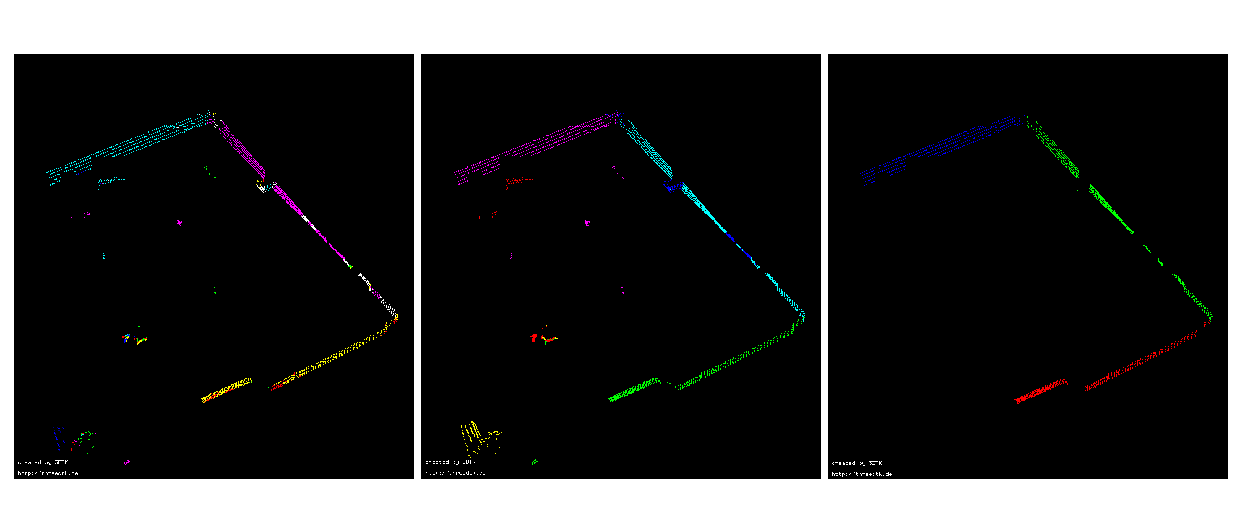
\includegraphics[width=\linewidth]{images/clustering}
	\caption{(Left) Point normals using the AKNN method with $K = 20$. (Middle) Result of the region growing, before applying the second filter. (Right) Resulting clusters after applying the second filter, using $N_{c,min} = 300$. }
	\label{fig:clustering}
\end{figure*}

Point-to-Plane correspondences are now established.
The distance models (Hesse and PPD) are utilized to check whether a cluster overlaps with any of the global planes, i.e. any point in the cluster has a Hesse distance smaller than some threshold $\epsilon_H$ and a PPD smaller than some additional threshold $\epsilon_P$, to the global plane.
For each overlap, we find the smallest angle between the corresponding cluster normal and the global plane normal, according to eq. \ref{eq:alphahat}.
Finally, a correspondence is established between all points in the cluster and the global plane, if the minimum angle between their normals is smaller than $\epsilon_\alpha$. 

\subsection{Optimization}

Assuming we now know the Hesse-normal form of all planes and all assigned points to these planes, we register the points to have a minimal distance to their respective planes.
The transformation $T(\vec{p}_i)$ of each point $\vec{p}_i$ with respect to a 6 DoF motion is described in homogeneous coordinates using the roll-pitch-yaw ($\varphi-\vartheta-\psi$) Tait-Brian angles as in~\cite{diebel2006representing}. Transforming the result back from homogeneous coordinates and using $C_a$ and $S_a$ to denote the cosine and sine of the angle in the subscript, and $t_a$ denoting the translation along the axis in the subscript yields:
\begin{align}
	T(\vec{p}_i)  =
    \resizebox{0.35\textwidth}{!}{$\begin{bmatrix}
        x_i C_\vartheta C_\psi - y_iC_\vartheta S_\psi + z_i S_\vartheta + t_x\\
        x_i (C_\varphi S_\psi + C_\psi S_\varphi S_\vartheta) + y_i(C_\varphi C_\psi - S_\varphi S_\vartheta S_\psi) - z_i C_\vartheta S_\varphi + t_y\\
        x_i(S_\varphi S_\psi - C_\varphi C_\psi S_\vartheta) + y_i(C_\psi S_\varphi + C_\varphi S_\vartheta S_\psi) + z_i C_\varphi C_\vartheta + t_z
    \end{bmatrix}$}
\end{align}
From this we define the function $D(\varphi,\vartheta,\psi,t_x,t_y,t_z, \vec{p}_i)$ that computes the distance of a point $\vec{p}_i$ to its corresponding plane $\mathcal{P}_k$.
Omitting the arguments of the function for simplicity:
\begin{align}
\begin{aligned}
    D &= T(\vec{p}_i) \cdot \vec{n}_{\mathcal{P}_k} \\
      &= n_{\mathcal{P}_k}^x (x_i C_\vartheta C_\psi - y_iC_\vartheta S_\psi + z_i S_\vartheta + t_x)\\
       &+ n_{\mathcal{P}_k}^y(x_i (C_\varphi S_\psi + C_\psi S_\varphi S_\vartheta)\\
       &\qquad+ y_i(C_\varphi C_\psi - S_\varphi S_\vartheta S_\psi) - z_i C_\vartheta S_\varphi + t_y)\\
       &+ n_{\mathcal{P}_k}^z (x_i(S_\varphi S_\psi - C_\varphi C_\psi S_\vartheta)\\
       &\qquad+ y_i(C_\psi S_\varphi + C_\varphi S_\vartheta S_\psi) + z_i C_\varphi C_\vartheta + t_z)\\
       &- \rho_{\mathcal{P}_k}
\end{aligned}
\end{align}

This distance function is what we want to minimize for all points and their respective planes.
Hence the error function $E$ is chosen as the square of the L2-norm of the distance:
\begin{align}
	E = \sum_{\forall \mathcal{P}_k}\sum_{\vec{p}_i \in \mathcal{P}_k} \norm[2]{D(\varphi,\vartheta,\psi,t_x,t_y,t_z, \vec{p}_i)}^2
\end{align}
Its gradient follows then immediately:
\begin{align}
	&\nabla E =  \sum_{\forall \mathcal{P}_k}\sum_{\vec{p}_i \in \mathcal{P}_k} \resizebox{0.28\textwidth}{!}{$\begin{bmatrix}\pardiff{\varphi} E&\pardiff{\vartheta} E&\pardiff{\psi} E&\pardiff{t_x} E&\pardiff{t_y} E&\pardiff{t_z} E\end{bmatrix}^T$}\\
    &\Rightarrow\nabla E = \resizebox{0.35\textwidth}{!}{$\sum_{\forall \mathcal{P}_k} \sum_{\vec{p}_i\in \mathcal{P}_k}2D(\vec{\Pi}, \vec{p}_i)\begin{bmatrix}\nabla E_\varphi &\nabla E_\vartheta & \nabla E_\psi & n_{\mathcal{P}_k}^x&n_{\mathcal{P}_k}^y&n_{\mathcal{P}_k}^z\end{bmatrix}^T$}
\end{align}
Where
\begin{align}
    &\begin{alignedat}{3}
        \nabla E_\varphi = &n_{\mathcal{P}_k}^y&&(x_i[-S_\varphi S_\psi+C_\varphi C_\psi S_\vartheta] \\&&&+y_i[-S_\varphi C_\psi -C_\varphi S_\vartheta S\psi] \\&&&- z_i C_\varphi C_\vartheta)\\
        &+ n_{\mathcal{P}_k}^z&&(x_i[C_\varphi S_\psi+C_\varphi C_\psi S_\vartheta] \\&&&+y_i[C_\varphi C_\psi -S_\varphi S_\vartheta S\psi] \\&&&- z_i S_\varphi C_\vartheta)
    \end{alignedat} \\
    &\begin{alignedat}{3}
        \nabla E_\vartheta = & n_{\mathcal{P}_k}^x(-x_iS_\vartheta C_\psi + y_i S_\vartheta S_\psi + z_iC_\vartheta) \\
        &+ n_{\mathcal{P}_k}^y(x_iC_\psi S_\varphi C_\vartheta - y_iS_\varphi C_\vartheta S_\psi + z_i S_\vartheta S_\varphi)  \\
        &+ n_{\mathcal{P}_i}^z(-x_iC_\varphi C_\psi C_\vartheta + y_iC_\varphi C_\vartheta S_\psi - z_i C_\varphi S_\vartheta)
    \end{alignedat}\\
    &\begin{alignedat}{3}
       \nabla E_\psi =& n_{\mathcal{P}_k}^x&&\left(-x_iC_\vartheta S_\psi - y_iC_\vartheta C_\psi\right) \\
       &+ n_{\mathcal{P}_k}^y&&(x_i[C_\varphi C_\psi - S_\varphi S_\vartheta S_\psi] \\
       &&&+ y_i[-C_\varphi S_\psi - S_\varphi S_\theta C_\psi]) \\
       &+ n_{\mathcal{P}_k}^z&&(x_i[S_\varphi C_\psi + C_\varphi S_\psi S_\theta] \\
       &&&+ y_i[-S_\psi S_ \varphi + C_\varphi S_\vartheta C_\psi]) 
    \end{alignedat}
\end{align}
and $\vec{\Pi}=\begin{bmatrix}\varphi & \vartheta & \psi & t_x & t_y & t_z\end{bmatrix}^T$.

As the gradient is well-defined we minimize the error function with any gradient based method. 
The commonly used, well-known stochastic gradient descent (SDG) algorithm computes 
\begin{align}
    \vec{\Pi}_{k+1} = \vec{\Pi}_{k} - \alpha \nabla E
\end{align}
where $\alpha$ is the learning rate.
To accelerate convergence and to improve the found solution further modifications are made.

Since we have vastly different effects on the error function by each dimension, the first consideration for improving the SDG is the following:
Typically, changes in orientation, i.e., the first three elements of the gradient vector $\pardiff{\varphi}E$, $\pardiff{\vartheta}E$, and $\pardiff{\psi}E$, have much more impact on the error function than a change in position.
This is intuitively explained since translating the scan makes the error grow linearly for all points.
However, when rotating the scan, points with a larger distance to the robot are moved drastically, leading to a higher sensibility on the error function.
For this reason, the $\alpha$ applied on orientation has to be much smaller than the $\alpha$ applied on the position.
It becomes obvious that $\alpha$ needs to be extended into vector form, $\boldsymbol\alpha$, therefore weighting each dimension differently.

Another consideration to speed up SDG is to adaptively recalculate $\boldsymbol\alpha$ for each iteration. 
We employ and modify ADADELTA as a technique to do so, which is described in detail in~\cite{zeiler2012adadelta}.
The main idea is the following:
It extends the SDG algorithm by two terms.
First, an exponentially decaying average of past gradients $\vec{G}_k$, which is recursively defined as
\begin{align}
    \vec{G}_{k+1} = \zeta \vec{G}_{k} + (1 - \zeta) {\nabla E}^2
\end{align}
and second, an exponentially decaying average of past changes $\vec{X}_k$, which is defined as
\begin{align}
    \vec{X}_{k+1} = \zeta \vec{X}_{k} + (1 - \zeta) {\boldsymbol\alpha \nabla E}^2
\end{align}
where $\zeta \leq 1$ is a decay constant, typically close to $1$.
The root mean squared (RMS) of these quantities are
\begin{align}
    RMS[\vec{G}]_{k} = \sqrt{\vec{G}_{k} + \epsilon_{num}}
\end{align}
and 
\begin{align}
    RMS[\vec{X}]_{k} = \sqrt{\vec{X}_{k} + \epsilon_{num}}
\end{align}
where $\epsilon_{num} > 0$ is a very small constant, typically close to $0$ (Note: this is a different threshold as the one used in section~\ref{sec:point-to-plane-correspondences}).
It will prevent dividing by zero in the recalculation of $\boldsymbol\alpha$, which is as follows:
\begin{align}
    \boldsymbol\alpha_{k} = \frac{RMS[X]_{k-1}}{RMS[G]_{k}}
    \label{eq:adadeltaalphaupdate}
\end{align} 
For our particular application, ADADELTA behaves a little too aggressively.
Despite giving a good measure on how to adapt $\boldsymbol\alpha$, the algorithm sometimes overshoots, and does not converge.
Therefore, we employ another scaling factor, typically not found in ADADELTA, extending eq.~\eqref{eq:adadeltaalphaupdate} to:
\begin{align}
    \boldsymbol\alpha_{k} = \boldsymbol\alpha_0 \cdot \frac{RMS[X]_{k-1}}{RMS[G]_{k}}
    \label{eq:adafinalized}
\end{align} 
where $\boldsymbol\alpha_0 $ holds the scaling factors for each dimension.

Finally, the SDG model is improved using eq.~\eqref{eq:adafinalized} and extends to 
\begin{align}
    \vec{\Pi}_{k+1} = \vec{\Pi}_{k} - \boldsymbol\alpha_0  \frac{RMS[X]_{k-1}}{RMS[G]_{k}} \cdot \nabla E
\end{align}
Using this algorithm once after finding correspondences from points to planes leads to convergence to a local minimum, which is often not an optimal solution.
Even if we increase the number of iterations dramatically, no better solution than the local minimum is found.
That is unless you consider updating the correspondence model after $i$ iterations of gradient descent.
Re-assigning point-to-plane correspondences this way $k$ times, with a large enough $k$, leads to an optimal solution after maximum $n = k\cdot i$ iterations of gradient descent.

\subsection{Further Optimizations of the Algorithm}

The algorithm was extended by two further optimizations, which are helpful in different scenarios.

Firstly, we introduce the possibility to choose a lock on some dimensions from being optimized by setting the corresponding $\alpha_i$ to zero.
Although 6D optimization generally works, reducing the optimization space is particularly useful if the source of error in the system is known and a model exists.
That way, e.g., as we expect a spherical robot to move on a plane the position along the axis perpendicular to the plane is constant and should not be used for optimization.\todo{@Fabi clarify in experiments which locks were active.} 

Secondly, we employ a continuous iteration, where the scans are processed sequentially. 
This is especially useful for mobile systems, where pose errors accumulate due to increasing tracking uncertainties.
The assumption is that the error in one scan is also present in the following scan, plus some unknown new error.
We eliminate the error from scan $m$ which is also present in scan $m+1$ by applying the pose change from scan $m$, $\vec{\Pi}_{n,m} - \vec{\Pi}_{0,m}$ after $n$ gradient descent iterations, to scan $m+1$, before restarting gradient descent.
